\documentclass[conference]{IEEEtran}

\IEEEoverridecommandlockouts

\usepackage{cite}
\usepackage{amsmath,amssymb,amsfonts}
\usepackage{graphicx}
\usepackage{textcomp}
\usepackage{xcolor}
\usepackage{listings}
\usepackage{xurl}
\usepackage{hyperref}
\usepackage{booktabs}
\usepackage{float}
\usepackage{tikz}
\usetikzlibrary{arrows.meta, positioning, shapes.geometric}

\definecolor{codegreen}{rgb}{0,0.6,0}
\definecolor{codegray}{rgb}{0.5,0.5,0.5}
\definecolor{codepurple}{rgb}{0.58,0,0.82}
\definecolor{backcolour}{rgb}{0.95,0.95,0.92}

\lstdefinestyle{mystyle}{
    backgroundcolor=\color{backcolour},
    commentstyle=\color{codegreen},
    keywordstyle=\color{magenta},
    numberstyle=\tiny\color{codegray},
    stringstyle=\color{codepurple},
    basicstyle=\ttfamily\footnotesize,
    breakatwhitespace=false,
    breaklines=true,
    captionpos=b,
    keepspaces=true,
    numbers=left,
    numbersep=5pt,
    showspaces=false,
    showstringspaces=false,
    tabsize=2
}
\lstset{style=mystyle}

\title{Bridging the Gap: \\Microcontroller Flashing on Android via Termux}

\author{
    \IEEEauthorblockN{Jnanesh Sathisha Karmar, Vivek K Kumar, \\
    Dr. G.V.V. Sharma}
    \IEEEauthorblockA{Department of Electrical Engineering, \\Indian Institute of Technology Hyderabad,\\ Kandi, India 502284 \\ gadepall@ee.iith.ac.in}
}

\begin{document}

\maketitle

% ─────────────────────────────────────────────────────────────
\begin{abstract}
This work addresses a fundamental limitation of the Android operating system: the absence of accessible, native hardware serial drivers for common microcontrollers. Without modifying the Java Native Interface (JNI) or requiring root access, the presented solution creates a robust user-space bridge that enables standard flashing tools—such as \texttt{avrdude} and \texttt{esptool.py}—to program physical microcontrollers and FPGAs over USB directly from a Termux terminal. The architecture centres on a heavily modified C++ pseudo-terminal shim (\textit{ptyserial}) that routes data through a standard pseudo-terminal while forwarding hardware control signals over a UNIX domain socket. An \texttt{LD\_PRELOAD} shared library intercepts critical system calls at runtime, preserving exact DTR/RTS toggle timing with microsecond precision. The system was successfully validated across CH340, FTDI, and CDC-ACM based Arduino boards, the ESP32, and a TinyFPGA B-Series (Vaman) board.
\end{abstract}

% ─────────────────────────────────────────────────────────────
\section{Introduction}

The proliferation of Android devices as capable computing platforms has opened new avenues for embedded systems development in the field. However, the Android operating system imposes a significant barrier: it does not expose standard serial port abstractions (e.g., \texttt{/dev/ttyUSB*}) for USB-attached microcontrollers without either root access or modifications to the Java Native Interface (JNI). This prevents developers from using mature, unmodified flashing tools—such as \texttt{avrdude} or \texttt{esptool.py}—directly on Android hardware.

This paper presents a fully user-space solution built on top of the Termux Linux environment for Android. The core contribution is a re-engineered \textit{ptyserial} C++ shim that elegantly bridges standard Linux serial software and physical USB hardware, together with an \texttt{LD\_PRELOAD} intercept library that transparently redirects hardware control system calls. The result is a universal, plug-and-play serial bridge requiring no root, no kernel patches, and no modification to the target flashing tool.

The foundation of this project is a fork of MarkWiims' Termux serial repository\cite{markwiims}, specifically incorporating CDC-ACM drivers added by GitHub user \textit{skikozou} (\texttt{skikozou/Termux-serial-tty}) \cite{skikozou}. Building upon this base, the core architecture was completely overhauled and heavily modified to achieve the described functionality.

The remainder of this paper is organised as follows. Section~\ref{sec:background} describes the relevant background. Section~\ref{sec:architecture} details the system architecture. Section~\ref{sec:kernel} explains how Android kernel limitations are circumvented. Section~\ref{sec:preload} describes the \texttt{LD\_PRELOAD} intercept mechanism. Section~\ref{sec:results} presents validation results. Section~\ref{sec:conclusion} concludes.

% ─────────────────────────────────────────────────────────────
\section{Background}
\label{sec:background}

\subsection{The Android USB Subsystem and Its Limitations}

Android's USB subsystem is designed primarily for host peripherals such as keyboards and storage devices. While it provides a \texttt{UsbManager} API for application-layer USB access, this API is Java-based and tightly coupled to the Android application model. The kernel can typically identify only its natively supported drivers—most notably CDC-ACM—when queried via the \texttt{USBDEVFS\_GETDRIVER} system call. Widely used serial bridge chips such as the CH340, FTDI FT232, and CP2102 are not natively recognised, making OS-assisted chip identification impossible without root.

Furthermore, because standard POSIX serial port paths (\texttt{/dev/ttyUSB*}, \texttt{/dev/ttyACM*}) are absent in a non-rooted Android environment, unmodified flashing tools that expect a physical COM port cannot operate.

\subsection{Termux and User-Space USB Access}

Termux~\cite{termux} is an Android terminal emulator and Linux environment that does not require root access. It provides a package ecosystem that includes development tools, compilers, and—critically—\texttt{libusb}, the cross-platform user-space USB library. \texttt{libusb}~\cite{libusb} allows applications to communicate directly with USB devices by claiming interfaces from user space, bypassing the kernel driver entirely. This capability is the foundation upon which the present architecture is built.

\subsection{Pseudo-Terminals}

A pseudo-terminal (PTY) \cite{posixpty} is a pair of virtual character devices—a master and a slave—that together provide an interface identical to a real terminal. The slave end (e.g., \texttt{/dev/pts/3}) appears to applications as a standard serial port. Data written to the master appears on the slave and vice versa. PTYs are widely used in terminal emulators and are the mechanism by which \textit{ptyserial} exposes a virtual COM port to unmodified flashing tools.

% ─────────────────────────────────────────────────────────────
\section{System Architecture}
\label{sec:architecture}

\subsection{Overview}

The system architecture is structured as a pipeline with two parallel channels: a high-speed \textit{data channel} for serial payload bytes, and a low-latency \textit{control channel} for hardware line signals. This strict separation ensures that DTR/RTS toggle operations do not corrupt or delay the primary data stream.

\begin{figure}[H]
\centering
\resizebox{0.95\columnwidth}{!}{%
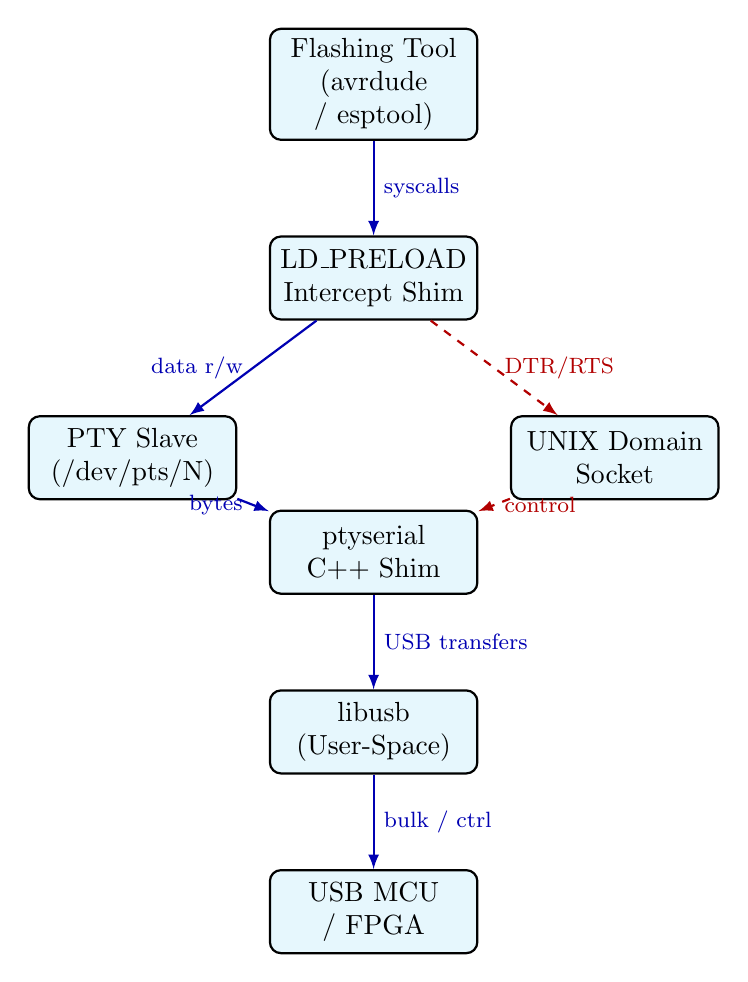
\begin{tikzpicture}[
  node distance=1.4cm and 1.2cm,
  auto,
  block/.style={
    rectangle, draw, fill=cyan!10,
    text width=2.4cm, text centered,
    rounded corners, minimum height=3em, line width=0.8pt
  },
  line/.style={draw, -latex, thick, color=blue!70!black},
  dashedline/.style={draw, -latex, thick, dashed, color=red!70!black}
]

  \node [block] (tool) {Flashing Tool\\(avrdude / esptool)};
  \node [block, below=1.2cm of tool] (shim) {LD\_PRELOAD\\Intercept Shim};
  \node [block, below left=1.2cm and 0.4cm of shim] (pty) {PTY Slave\\(/dev/pts/N)};
  \node [block, below right=1.2cm and 0.4cm of shim] (sock) {UNIX Domain\\Socket};
  \node [block, below=2.4cm of shim] (ptyserial) {ptyserial C++ Shim};
  \node [block, below=1.2cm of ptyserial] (libusb) {libusb\\(User-Space)};
  \node [block, below=1.2cm of libusb] (mcu) {USB MCU / FPGA};

  \path [line] (tool) -- node[right, font=\footnotesize]{syscalls} (shim);
  \path [line] (shim) -- node[left, font=\footnotesize]{data r/w} (pty);
  \path [dashedline] (shim) -- node[right, font=\footnotesize]{DTR/RTS} (sock);
  \path [line] (pty) -- node[left, font=\footnotesize]{bytes} (ptyserial);
  \path [dashedline] (sock) -- node[right, font=\footnotesize]{control} (ptyserial);
  \path [line] (ptyserial) -- node[right, font=\footnotesize]{USB transfers} (libusb);
  \path [line] (libusb) -- node[right, font=\footnotesize]{bulk / ctrl} (mcu);

\end{tikzpicture}
}
\caption{Full system pipeline. Solid arrows indicate data flow; dashed arrows indicate out-of-band hardware control signals.}
\label{fig:pipeline}
\end{figure}

\subsection{The ptyserial Dual-Channel Architecture}

When a USB device is plugged in, the Android kernel typically attaches its own limited drivers to it. The \textit{ptyserial} shim uses \texttt{libusb} to forcefully detach the kernel driver and explicitly claim the USB interface for user-space control.

Data bytes are seamlessly piped back and forth through a standard pseudo-terminal (e.g., \texttt{/dev/pts/3}), allowing unmodified software to read and write data as if communicating with a physical COM port. \cite{unixsocket} Simultaneously, a dedicated UNIX domain socket runs in parallel as an out-of-band control channel. This socket waits to accept real-time hardware requests, keeping the primary data stream fast and uncorrupted.

The elegance of this dual-channel architecture lies in its strict separation of concerns: high-speed serial data never shares a path with low-frequency hardware control signals, eliminating any possibility of timing interference.

% ─────────────────────────────────────────────────────────────
\section{Overcoming Android Kernel Limitations}
\label{sec:kernel}

\subsection{The VID:PID Identification Problem}

A significant hurdle in Android's USB subsystem is driver identification. The kernel can accurately report its native drivers (such as CDC-ACM) when queried via \texttt{USBDEVFS\_GETDRIVER}, but it lacks native awareness of other common serial bridge silicon. Relying on the OS to identify the chip is therefore not a viable strategy.

\subsection{Hardcoded VID:PID Table}

To bypass this limitation, the architecture employs a hardcoded Vendor ID and Product ID (VID:PID) lookup table within the user-space shim. By manually matching the USB hardware identifiers against this internal table, the system can instantly identify and load the correct configurations for popular chips, completely circumventing the Android kernel's blind spots.

\begin{table}[H]
\centering
\caption{Supported chipsets via VID:PID table}
\label{tab:chips}
\begin{tabular}{@{}lll@{}}
\toprule
\textbf{Chip} & \textbf{VID} & \textbf{Common Use} \\
\midrule
CH340 / CH341 & 0x1A86 & Arduino Nano clones \\
FTDI FT232    & 0x0403 & Arduino Uno, custom boards \\
CP2102        & 0x10C4 & ESP8266, ESP32 modules \\
CDC-ACM       & 0x2341 & Official Arduino, native path \\
\bottomrule
\end{tabular}
\end{table}

% ─────────────────────────────────────────────────────────────
\section{The LD\_PRELOAD Intercept Mechanism}
\label{sec:preload}

\subsection{Motivation}

Standard flashing tools expect a physical serial port and will crash or malfunction when their hardware control commands (such as \texttt{tcdrain} or \texttt{ioctl}) are directed at a virtual pseudo-terminal. Modifying each flashing tool to handle PTYs gracefully is impractical and defeats the goal of a universal solution. Instead, an \texttt{LD\_PRELOAD} shared library is injected at runtime to intercept these system calls before they reach the OS.

\subsection{Intercepted System Calls}

Table~\ref{tab:intercepts} summarises the system calls intercepted by the shim and the corresponding action taken.

\begin{table}[H]
\centering
\caption{System call interception behaviour}
\label{tab:intercepts}
\begin{tabular}{@{}p{2.2cm}p{4.8cm}@{}}
\toprule
\textbf{System call} & \textbf{Action} \\
\midrule
\texttt{TIOCMGET} & Block OS call; return locally tracked modem state (\texttt{g\_modem\_bits}). \\
\addlinespace
\texttt{TIOCMSET}\newline\texttt{TIOCMBIS}\newline\texttt{TIOCMBIC} & Intercept command; forward new DTR and RTS states directly to the UNIX domain socket for physical USB control transfer. \\
\addlinespace
\texttt{TIOCEXCL}\newline\texttt{TIOCNXCL} & Silently return 0 (success); tool believes port is exclusively locked. \\
\addlinespace
\texttt{flock} & Silently return 0; bypasses file-lock requirement on virtual PTY. \\
\addlinespace
\texttt{tcdrain} & Return 0; prevents crash on virtual PTY. \\
\bottomrule
\end{tabular}
\end{table}

\subsection{State Management}

The shim maintains a local integer \texttt{g\_modem\_bits} that shadows the logical state of the hardware modem lines (DTR, RTS, CTS, DSR, etc.). When a tool queries the line state via \texttt{TIOCMGET}, the shim returns this locally tracked value rather than forwarding the call to the kernel—which would fail on a PTY. When a tool asserts or clears hardware lines via \texttt{TIOCMSET}, \texttt{TIOCMBIS}, or \texttt{TIOCMBIC}, the shim updates \texttt{g\_modem\_bits} and simultaneously writes the new DTR/RTS state to the UNIX socket, triggering a real USB control transfer in \textit{ptyserial}.

\begin{figure}[H]
\centering
\resizebox{0.95\columnwidth}{!}{%
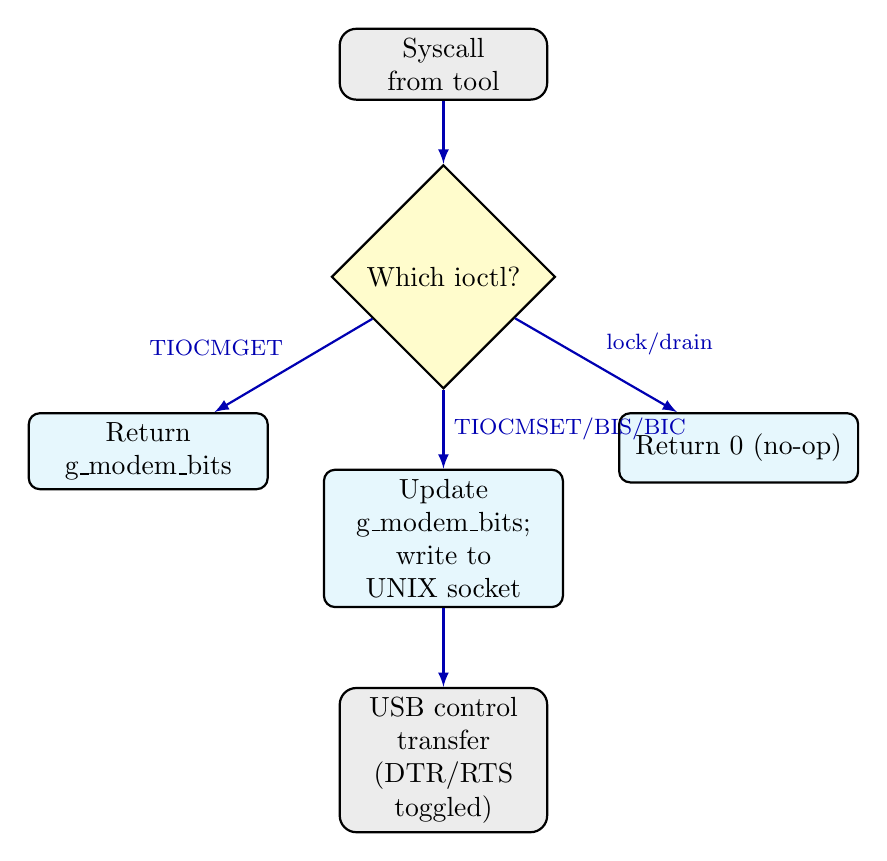
\begin{tikzpicture}[
  node distance=1.3cm and 1.0cm,
  auto,
  decision/.style={
    diamond, draw, fill=yellow!20,
    text width=2.6cm, text centered,
    inner sep=0pt, minimum height=2.5em, line width=0.8pt
  },
  block/.style={
    rectangle, draw, fill=cyan!10,
    text width=2.8cm, text centered,
    rounded corners, minimum height=2.5em, line width=0.8pt
  },
  term/.style={
    rectangle, draw, fill=gray!15,
    text width=2.4cm, text centered,
    rounded corners=6pt, minimum height=2em, line width=0.8pt
  },
  line/.style={draw, -latex, thick, color=blue!70!black}
]

  \node [term] (entry) {Syscall from tool};
  \node [decision, below=0.8cm of entry] (which) {Which ioctl?};
  \node [block, below left=1.0cm and 1.5cm of which] (mget) {Return g\_modem\_bits};
  \node [block, below=1.0cm of which] (mset) {Update g\_modem\_bits;\\ write to UNIX socket};
  \node [block, below right=1.0cm and 1.5cm of which] (ignore) {Return 0 (no-op)};
  \node [term, below=1.0cm of mset] (usb) {USB control transfer\\ (DTR/RTS toggled)};

  \path [line] (entry) -- (which);
  \path [line] (which) -- node[above left, font=\footnotesize]{TIOCMGET} (mget);
  \path [line] (which) -- node[right, font=\footnotesize]{TIOCMSET/BIS/BIC} (mset);
  \path [line] (which) -- node[above right, font=\footnotesize]{lock/drain} (ignore);
  \path [line] (mset) -- (usb);

\end{tikzpicture}
}
\caption{LD\_PRELOAD intercept decision flow.}
\label{fig:intercept}
\end{figure}

% ─────────────────────────────────────────────────────────────
\section{Validation and Results}
\label{sec:results}

\subsection{Hardware Tested}

The architecture was validated across a representative range of hardware spanning all three driver categories present in the VID:PID table.

\begin{itemize}
  \item \textbf{CH340-based Arduino boards} (e.g., Arduino Nano clone): Sketch upload via \texttt{avrdude}, including the DTR-triggered auto-reset cycle.
  \item \textbf{FTDI-based Arduino boards}: Full firmware upload with correct baud rate negotiation.
  \item \textbf{CDC-ACM Arduino boards}: Native driver path exercised through the same unified interface.
  \item \textbf{ESP32 (CP2102)}: \texttt{esptool.py flash\_id} command and full firmware flash with the EN/IO0 reset sequence triggered via RTS/DTR toggling.
  \item \textbf{TinyFPGA B-Series (Vaman board)}: Bitstream upload, which relies on a precise, multi-step RTS/DTR reset sequence with strict inter-signal timing.
\end{itemize}

\subsection{Timing Preservation}

The most demanding test case was the TinyFPGA B-Series, whose bootloader requires a specific sequence of DTR and RTS transitions with microsecond-level timing. By intercepting the exact moment the flashing tool requested a DTR/RTS toggle and immediately routing it via the UNIX socket to physical USB control transfers, the system natively preserved the exact timing intended by the original tool developers.

This result demonstrates a key architectural advantage: because the interception occurs at the system-call boundary—where the tool issues the hardware command—rather than at an emulated baud-rate clock, the timing fidelity is determined by the tool itself, not by the bridge. The bridge simply relays the command to hardware as fast as the USB subsystem permits.

\subsection{Universality}

This elegant interception approach completely bypassed the need to reverse-engineer and write custom DTR/RTS reset sequences for each microcontroller family. Any future device whose reset protocol is already implemented in a standard flashing tool will work automatically, without modification to the bridge.

% ─────────────────────────────────────────────────────────────
\section{Conclusion}
\label{sec:conclusion}

This work presented a user-space serial bridge for Android that enables standard, unmodified microcontroller flashing tools to program USB-attached hardware from within the Termux environment—without root access, kernel modifications, or JNI changes. The architecture combines three cooperating components: (1) the \textit{ptyserial} C++ shim, which uses \texttt{libusb} to claim USB interfaces and exposes a PTY as a virtual COM port; (2) a UNIX domain socket serving as an out-of-band control channel for DTR/RTS signals; and (3) an \texttt{LD\_PRELOAD} intercept library that transparently redirects hardware control system calls from the flashing tool into the bridge pipeline.

Successful validation across CH340, FTDI, CDC-ACM, CP2102, and custom bootloader targets demonstrates that the system is genuinely universal. The timing-preserving interception architecture eliminates per-device customisation and positions the bridge as a drop-in solution for any hardware whose flashing protocol is already supported by an existing tool.

Future work includes expanding the VID:PID table, adding automated baud-rate detection, and exploring integration with Mission Planner for ArduPilot firmware deployment from Android.

% ─────────────────────────────────────────────────────────────
\bibliographystyle{IEEEtran}
\bibliography{references}

\end{document}
